% Navigation: unnumbered; does not consume the appendix letter A.
\section*{Guide to the Supplement}
Sections A--B examine the two central design choices: the strength of adaptation and the source of a missing grade's displacement.
The remaining sections establish how transfer depends on supervision, extend the evaluation, and provide the derivations and protocols.

\noindent\begin{tabularx}{\columnwidth}{@{}lX@{}}
\textbf{A} & Global blending and classification trade-offs.\\
\textbf{B} & Reference preservation and displacement inheritance.\\
\textbf{C} & Grade support, missing patterns, and full support.\\
\textbf{D} & Adaptation regimes, backbones, and domains.\\
\textbf{E} & Derivations and the inference algorithm.\\
\textbf{F} & Configurations, prompts, and evaluation protocols.
\end{tabularx}

\noindent The central comparisons are in Secs.~\ref{sec:supp_best_blend}--\ref{sec:supp_error_tradeoffs} and \ref{sec:supp_keep_inherit}; Sec.~\ref{sec:supp_inheritance_error} explains the remaining inheritance error.

\section{Beyond Global Blending}
\label{sec:supp_blending}

TIE changes the source of a missing grade's adaptation; global blending changes its strength.
We examine this distinction across adapter configurations and at the best evaluated blending strength, then compare the resulting classification trade-offs.

\subsection{Configuration-Level Ranking Curves}
\label{sec:supp_config_curves}

Let $T$ and $S$ denote the zero-shot and adapted scores, and let $D=S-T$.
Global score blending provides an output-space counterpart to zero-shot/fine-tuned weight interpolation~\cite{wortsman2022robust}.
At strength $\lambda$, the two score constructions are
\begin{equation}
\begin{aligned}
 B_\lambda &= T+\lambda D,\\
 S^{\mathrm{TIE}}_\lambda &= T+\lambda\mathcal L_{\mathcal U}(D).
\end{aligned}
\label{eq:supp_matched_paths}
\end{equation}
Here $\mathcal U$ is the set of missing grades and $\mathcal L_{\mathcal U}$ is the inheritance operator from the main paper.
At every matched strength, the two constructions have identical seen-grade scores and differ only in the missing grades' displacement.
Class-bias calibration preserves their respective pairwise rankings by Proposition~1 of the main paper.

Sections~A.1--A.2 use the three interior missing-grade masks and three seeds for each of the nine adapter configurations.
Each configuration curve therefore averages nine conditions; the dataset mean averages all nine configurations equally, for 81 conditions per dataset.
We evaluate $\lambda\in\{0,0.1,\ldots,1.5,2.0\}$.
The zero-shot reference is recovered at $\lambda=0$, $\lambda=1$ retains the original adaptation strength, and $\lambda>1$ extrapolates.
MS-AUC averages pair AUROC over adjacent missing--seen grade pairs.

Figure~\ref{fig:supp_config_curves} resolves the difference between the two paths by configuration.
At $\lambda=1$, TIE improves MS-AUC in 35 of the 36 configuration--dataset settings: eight of nine on Adience and all nine on HCI, FairFace, and KonIQ.
This is the interior-mask counterpart of the 34/36 result over all six masks in the main paper.
The improvement spans the adaptation configurations, while the curves expose differences in its magnitude and dependence on strength.

\begin{figure*}[!t]
\centering
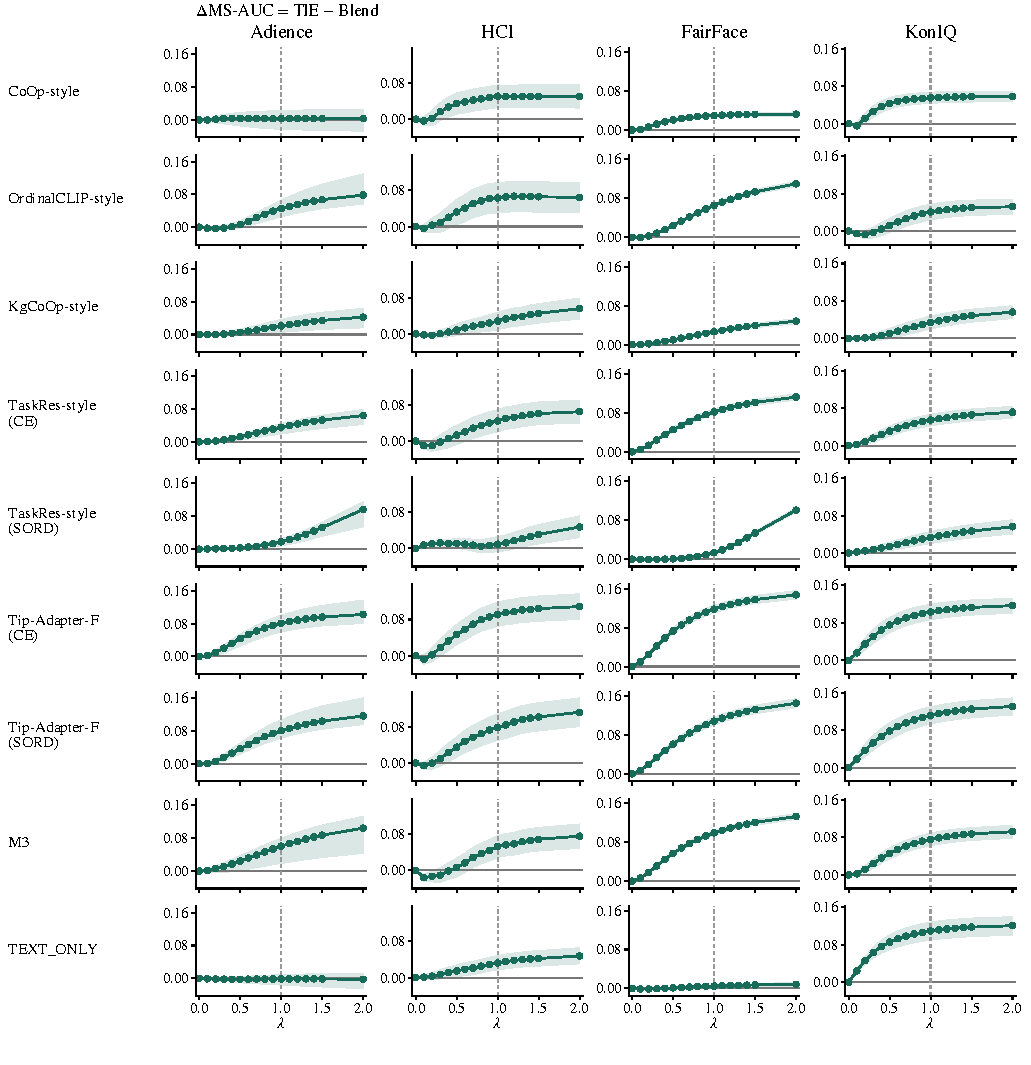
\includegraphics[width=\textwidth]{figures/supp/supp_a_configuration_curves.pdf}
\caption{\textbf{Ranking gains across configurations and strengths.}
Each panel shows $\Delta=\text{MS-AUC}(\text{TIE})-\text{MS-AUC}(\text{Blend})$ for one configuration and dataset, averaged over three interior masks and three seeds.
Points mark all 17 evaluated strengths; available paired pointwise 95\% bootstrap intervals are shaded.
Horizontal lines mark zero gain and vertical dashed lines mark $\lambda=1$.
All panels in a column share their vertical scale.
Configuration definitions are given in Sec.~F.2.}
\label{fig:supp_config_curves}
\end{figure*}

\subsection{Matched Strengths and the Best Evaluated Blend}
\label{sec:supp_best_blend}

At the original adaptation strength, TIE gains 0.038--0.069 MS-AUC over Blend (Table~\ref{tab:supp_best_blend}).
Across the grid, the paired 95\% interval is entirely positive at 59 of the 64 nonzero dataset--strength combinations: 14/16 on Adience, 13/16 on HCI, and 16/16 on both FairFace and KonIQ.
HCI at $\lambda=0.1$ is the only negative interval.
The intervals cross zero at $\lambda=0.1,0.2$ on Adience and $\lambda=0.2,0.3$ on HCI.

We next give Blend its best strength on the grid, chosen separately for each dataset using test MS-AUC and shared across all nine configurations.
TIE remains at $\lambda=1$.
On HCI, FairFace, and KonIQ, it exceeds even this best Blend by 0.042, 0.018, and 0.067, respectively.
TIE also exceeds the zero-shot reference on these three benchmarks by 0.113, 0.025, and 0.096.
Its gains therefore go beyond recovering the reference order.

\begin{table*}[t]
\centering
\caption{\textbf{Original-strength transfer versus the best global blend.}
Results use the interior masks and equal configuration weighting of the main paper's Fig.~2.
The confidence interval belongs to the paired difference at the fixed strength $\lambda=1$.
Best Blend maximizes dataset-mean test MS-AUC over the 17-point grid with one shared strength $\lambda^\star$; the final column reports TIE at $\lambda=1$ minus this best Blend.
Differences are computed before rounding.}
\label{tab:supp_best_blend}
\small
\begin{tabular*}{\textwidth}{@{\extracolsep{\fill}}lcccc@{}}
\toprule
Dataset & TIE$_1$ & TIE$_1$ $-$ Blend$_1$ [95\% CI]
 & Best Blend ($\lambda^\star$) & TIE$_1$ $-$ Best Blend\\
\midrule
Adience  & 0.906 & $+0.038\;[0.024,0.046]$ & 0.918 (0.1) & $-0.012$\\
HCI      & 0.742 & $+0.050\;[0.034,0.066]$ & 0.700 (0.5) & $\mathbf{+0.042}$\\
FairFace & 0.817 & $+0.061\;[0.058,0.064]$ & 0.800 (0.2) & $\mathbf{+0.018}$\\
KonIQ    & 0.635 & $+0.069\;[0.057,0.080]$ & 0.568 (0.6) & $\mathbf{+0.067}$\\
\bottomrule
\end{tabular*}
\end{table*}

Adience starts from a strong zero-shot ranking: 0.916 MS-AUC, compared with 0.867 after adaptation.
TIE at $\lambda=1$ reaches 0.906 and recovers 79\% of this loss.
From $\lambda=0$ to $2$, its MS-AUC decreases by 0.030, compared with 0.097 for Blend.
Here, transfer preserves much more of the reference ordering as adaptation strength increases.

\subsection{Missing--Seen Error Trade-offs}
\label{sec:supp_error_tradeoffs}

Figure~\ref{fig:supp_error_tradeoffs} places the six methods from Table~1 of the main paper in the plane of seen-grade and missing-grade MAE.
This comparison uses all six missing-grade masks, giving 162 conditions per dataset with equal weighting across configurations.
Within each condition, Missing MAE averages the per-grade errors over missing grades; Seen MAE averages errors over seen-grade test images.
Lower values on both axes are better.
The suffix +C denotes class-bias calibration.
Each calibrated method uses its own offset under the same seen-validation protocol.
Both Blend selectors use validation data; the test-set maximization in Sec.~A.2 serves only the ranking comparison.

\begin{figure*}[!t]
\centering
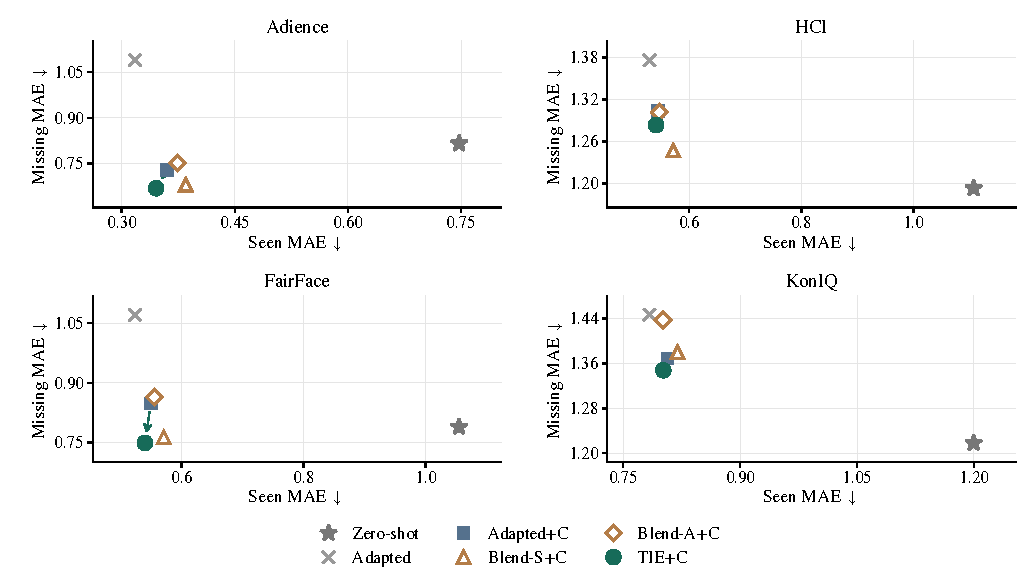
\includegraphics[width=\textwidth]{figures/supp/supp_a_error_tradeoff.pdf}
\caption{\textbf{Preserving adaptation while reducing missing-grade error.}
Each point is a method from Table~1 of the main paper, averaged over nine configurations, six masks, and three seeds.
Lower left is better.
Missing MAE is averaged across missing grades; Seen MAE is averaged across seen-grade images.
The green arrows connect Adapted+C to TIE+C.
The zero-shot point uses the reference scores for all grades.
Each dataset retains its own axis ranges.}
\label{fig:supp_error_tradeoffs}
\end{figure*}

TIE+C lowers both missing-grade and seen-grade MAE relative to Adapted+C on all four benchmarks.
Returning entirely to zero-shot produces a different trade-off.
On HCI, zero-shot has lower Missing MAE than TIE+C, 1.193 versus 1.284, but its Seen MAE is 1.108 versus 0.541.
KonIQ shows the same pattern: Missing MAE is 1.218 versus 1.348, while Seen MAE is 1.200 versus 0.802.
TIE retains the benefit of adaptation on seen grades while reducing the damage to missing grades.

HCI also exposes the trade-off between the calibrated methods.
Blend-S+C reaches lower Missing MAE than TIE+C, 1.247 versus 1.284, with higher Seen MAE, 0.571 versus 0.541.
TIE+C nevertheless has higher MS-AUC, 0.678 versus 0.639, and lower overall MAE, 0.772 versus 0.784.
Ranking and the final classification operating point therefore provide complementary evidence.

The zero-shot comparison above uses $T$ for every grade.
Keeping $T$ only for missing grades while retaining adapted seen-grade scores is a separate construction, examined in Sec.~B.1.
That section isolates the two ingredients of TIE: preserving a grade's own reference and inheriting its neighbors' displacement.
